
Some examples include sex, age, education level, socioeconomic status or marital status. Information collections with biased tendencies can't generate a representative sample.

Variables considered in the study must accurately reflect the populations characteristics. 

Consider \textit{attribute: income} of a subset of GBS participants. Statistical significance tests, e.g. Kolmogorov-Smirnov, Chi-Squared

\begin{figure}[ht]
	\begin{center}
		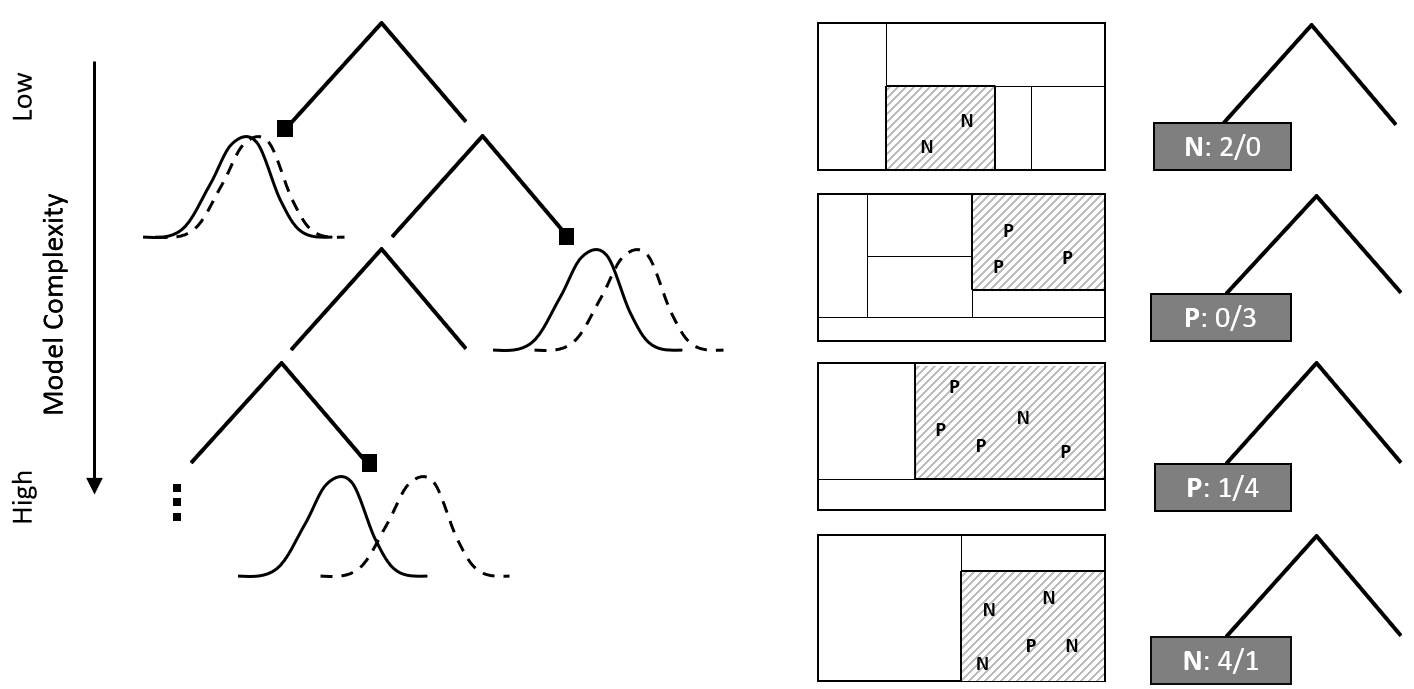
\includegraphics[scale=0.40,angle=0]{fig/tree3}
		\label{project}
		\caption{.}
	\end{center}
\end{figure}

Given a subset of GBS, similarity scores can be defined to evaluate the distance to reference distributions from GESIS. Kolmogorov-Smirnov tests or Chi-Squared assess the likelihood of an attribute of GBS  There are \(2^{|GBS|} = 2^{587}\) subsets of GBS. Evaluating every possible combination of GBS participants and its score is computationally intractable.

A well-defined learning problem where large polls (Umfragedaten) may contain valuable implicit regularities, requires a well-specified task, performance metric and source of training experience [2]. The MRS problem is now stated as a binary classification task with GESIS as positive class and GBS as negative class. Consider designing a computer program to learn to distinguish between . Using prior knowledge together with past experience to guide learning, a machine learning algorithm
is fed with data from games that have been played by chess grandmasters. From this information, the program will learn to apply certain functions to specific board states and make decisions about which move to play next.

Consider a randomly chosen survey participant, i.e. an instance of GBS or GESIS. If the poll indicates the or

Descriptive statistics can be used to 
 
No practical amount of data can distinguish between two distributions, thus instances of GBS can not be proven to come from GESIS. However, discriminative learning allows to infer the conditional probability of \textit{'instance of GBS/GESIS'} given the survey data within a probabilistic framework:

Discriminative learners will look for decision boundaries to distinguish the different views of GBS from GESIS. False negatives are then more closely aligned with the target probability distribution. The process of classification is repeated until the learner starts fitting noise more than is warranted. To avoid overfitting, the learning objective needs to be refined as contingency tables lack proper interpretibility. Given the imbalanced nature and size of GBS, learning is restrained to simpler algorithms with lesser degrees of freedom. The fraction of false positives in the result set of this procedure is kept as proxy measure for the subsequent method positive-unlabeled learning (PU learning). The development of classification models in this setting is often referred to as positive-unlabeled learning (Denis et al. 2005).

\begin{figure}[ht]
	\begin{center}
		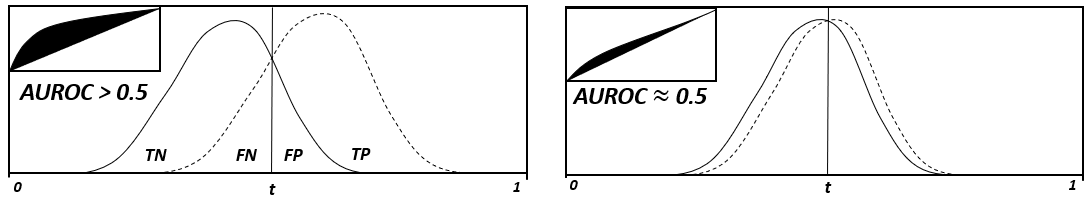
\includegraphics[scale=0.53,angle=0]{fig/roc_example}
		\label{project}
		\caption{There is no caption for such a stupid figure.}
	\end{center}
\end{figure}

PU learning is a semi-supervised technique that does not make the simplifying assumption of GBS instances being negative. Instead, a one-class classifier is trained on GESIS only. [...] This can result in even better assessment. [Read Literature] - Imporance weighted cross validation and pu learning with proper assessment.
